\section{Investimento residencial e a lacuna heterodoxa}
\label{Secao_Residencial}

%Tal como pontua \textcite{dipasquale_why_1999}, a discussão sobre os determinantes do \textit{preço} dos imóveis é mais ampla que do investimento residencial propriamente dito. 
Diante da lacuna empírica destacada anteriormente, esta seção busca ilustrar --- a começar pelos trabalhos ortodoxos --- a importância do investimento residencial para o crescimento e ciclo econômico. 
Cabe a essa seção, portanto, evidenciar algumas destas lacunas.
Neste ponto, cabe mencionar o ineditismo de \textcite{green_follow_1997} e \textcite{leamer_housing_2007} --- e revisitado em \textcite{leamer_housing_2015} e por \textcite{fiebiger_trend_2017} --- ao lançar luz sobre a importância do investimento residencial na determinação dos ciclos econômicos antes mesmo da crise dos \textit{subprimes}. 

%Desse modo, a literatura do supermultiplicador é um contraponto ao \textit{trade-off} apontado por \textcite{solow_importance_1995} uma vez que são os gastos autônomos que lideram o crescimento no longo prazo.
  
%TODO Rever conexão entre parágrafos.


Ao avaliar o caso norte-americano, \textcite{green_follow_1997} conclui que o investimento residencial possui uma capacidade preditiva maior que o investimento das firmas, mas que isso não implica no estabelecimento de uma relação causal. Na tentativa de compreender tais resultados, afirma:

\begin{citacao}

[P]erhaps residential investiment, like stock prices and interest rates, is a good predictor of GDP because it is a series that reflects \textbf{foward looking behavior}. Presumably households will not increase their expenditures on housing unless they expect to prosper in the future. Building a house is a natural mechanism for doing this. Thus, the series can do a good job of predicting GDP without necessarily causing GDP.
\cite[p.~267, grifos adicionados]{green_follow_1997}
\end{citacao}
Apesar de dar atenção para um gasto não criador de capacidade, o argumento de \textcite{green_follow_1997} se difere das conclusões do supermultiplicador uma vez que não são estes gastos que lideram o crescimento.
\textcite{leamer_housing_2007}, por sua vez, avança em direção a relação de causalidade entre este gasto e o PIB. Grosso modo, afirma que a construção de novos imóveis implica em maior consumo de bens duráveis e, portanto, trata-se de um ciclo decorrente do \textit{volume} e não do preço dos imóveis. 

Uma forma de visualizar a importância do investimento residencial para o ciclo econômico na economia estadunidense é por meio do gráfico \ref{Investo_Resid} em que cada um dos painéis apresenta um ciclo iniciado no primeiro trimestre de crescimento positivo após a recessão\footnote{
	Raciocínio semelhante pode ser encontrado em \textcite{fiebiger_semi-autonomous_2018} em que, diferentemente do presente trabalho, não é incluído consumo financiado por crédito.}. 
No eixo vertical, observa-se a participação desse gasto no PIB, enquanto no eixo horizontal, o grau de utilização da capacidade como uma \textit{proxy} para o ciclo econômico. Exceto para o período 1991-2001, a recuperação (aumento da utilização da capacidade) é caracterizada por uma taxa de crescimento do investimento residencial maior que o crescimento da economia, resultando em maior participação desse gasto no PIB. Considerando que as firmas seguem o princípio do ajuste do estoque de capital, ampliam a taxa de acumulação de modo a ajustar o grau de utilização para o grau normal. O aumento da taxa de crescimento do investimento das firmas e de outros gastos reduz a participação do investimento residencial no PIB. A maturação do investimento das firmas, por sua vez, redunda em menor utilização da capacidade produtiva\footnote{
	Complementarmente, os trabalhos de \textcite{fiebiger_semi-autonomous_2018} e \textcite{fiebiger_trend_2017} também reportam o investimento residencial como determinante do comportamento cíclico e adicionam o consumo financiado por crédito a essa dinâmica. Além disso, apresentam uma similaridade com \textcite{dejuan_hidden_2017} e \textcite{teixeira_crescimento_2015} para os quais a instabilidade econômica está associada à instabilidade (ao menos de alguns) gastos autônomos e não do investimento das firmas, que segue o princípio do ajuste do estoque de capital.}. 

%TODO Melhorar resolução gráfico e traduzir eixos

\begin{figure}[H]
	\centering
	\caption{Relação entre taxa de investimento residencial e grau de utilização por recessão}
	\label{Investo_Resid}
	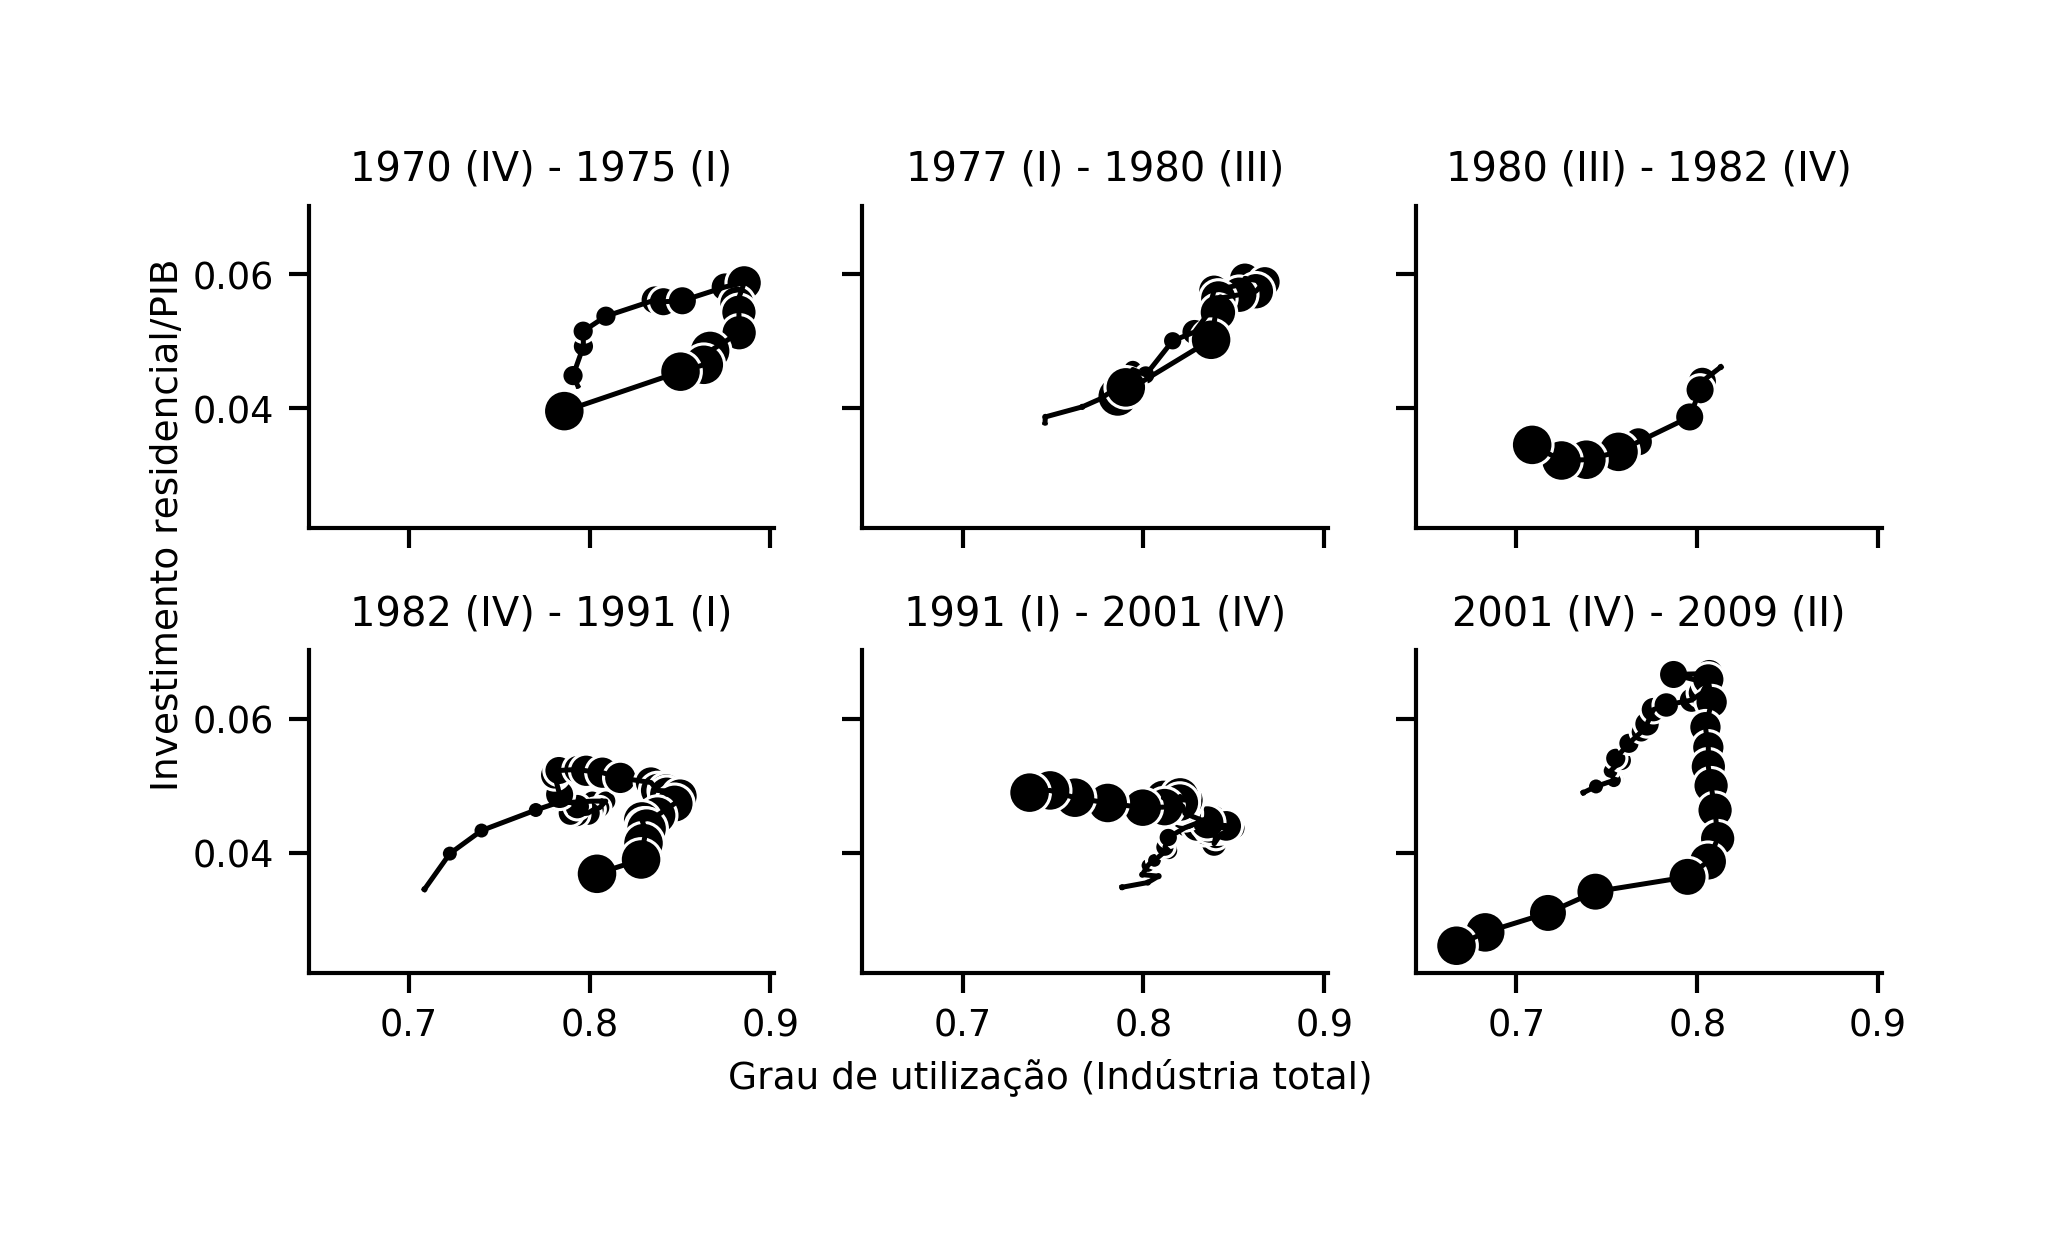
\includegraphics[width=\textwidth]{Fatos_Estilizados/Figs/Empiria.png}
	\caption*{\textbf{Fonte:} Elaboração própria}
\end{figure}

Desse modo, conclui-se que o investimento residencial ajuda a compreender grande parte das recessões e tal componente de gasto também é significativo para a retomada. Esta dinâmica poder ser visualizada no gráfico \ref{Recuperacao} em que são apresentadas algumas taxas de crescimento\footnote{Neste gráfico, as taxas de crescimento são normalizadas para facilitar a comparatibilidade uma vez que é mantida uma mesma escala.} nos trimestres que antecedem e sucedem as recuperações. Em linhas gerais, observa-se que o investimento residencial possui uma taxa de crescimento (a taxas crescentes) positiva nos trimestres que antecedem a recuperação enquanto o investimento das firmas só apresenta tal comportamento adiante. Portanto, esse gráfico ilustra tanto a capacidade do investimento residencial liderar a retomada quanto a indução do investimento criador de capacidade produtiva.

\begin{figure}[H]
	\centering
	\caption{Taxa de crescimento normalizada por recessões antes e depois do início da recuperação}
	\label{Recuperacao}
	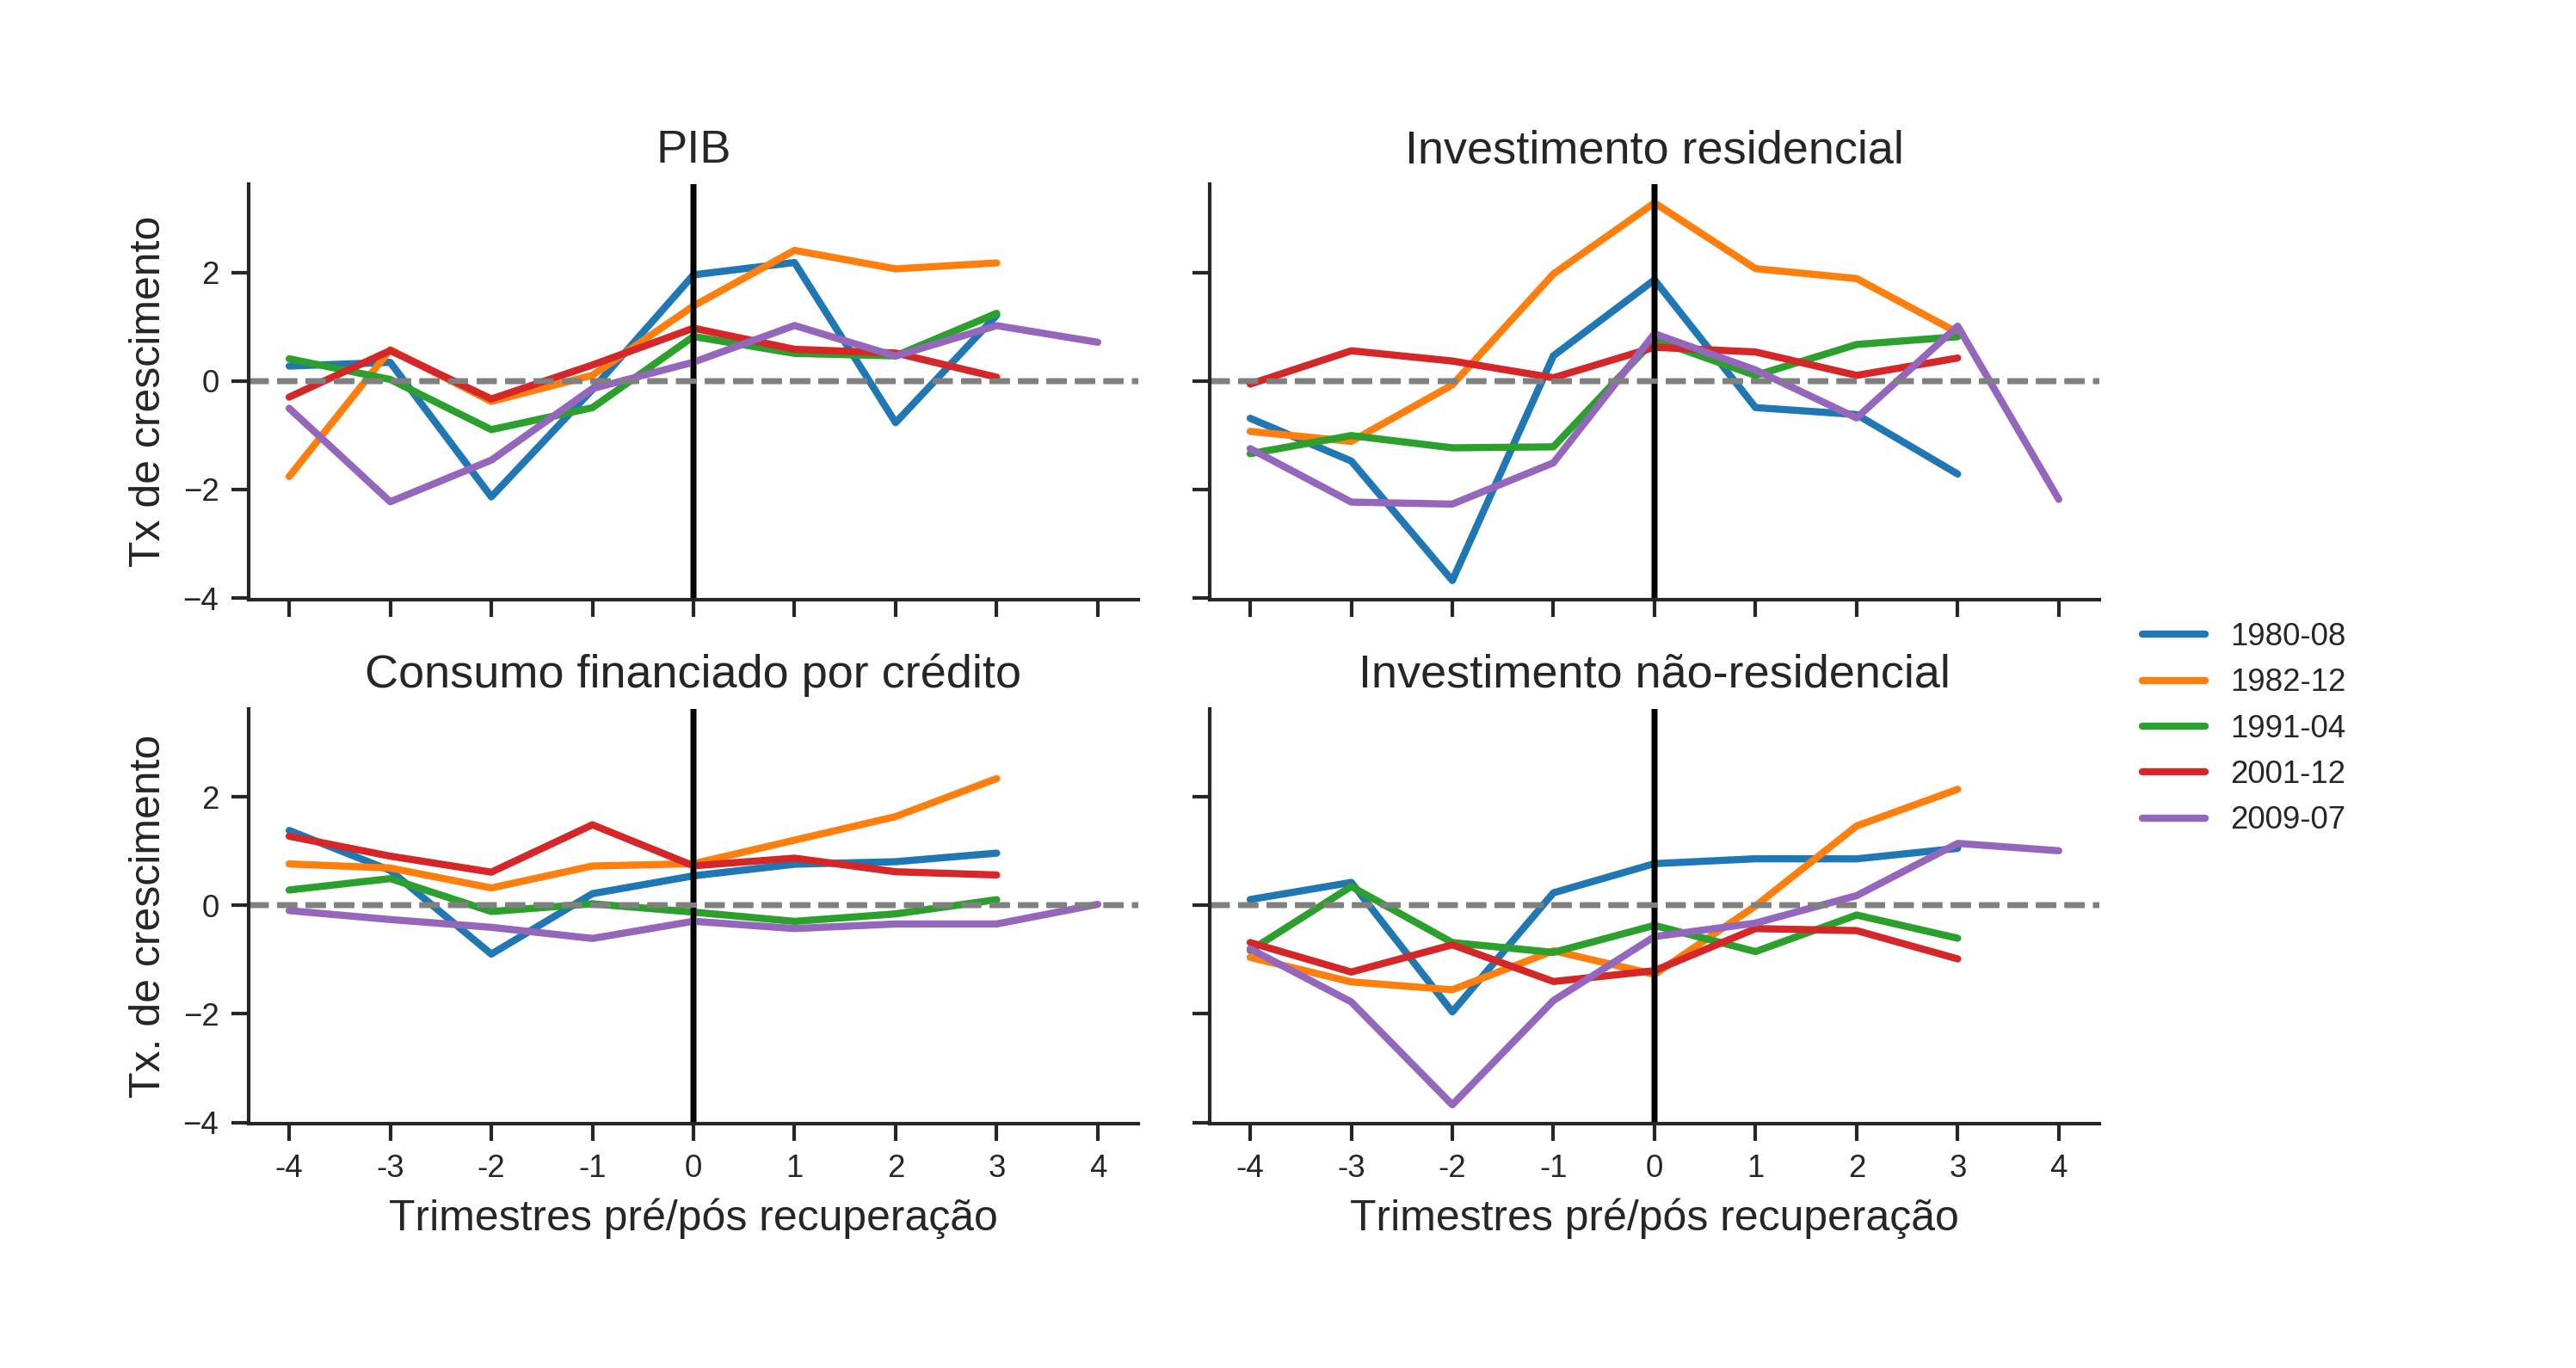
\includegraphics[width=\textwidth]{Fatos_Estilizados/Figs/Recuperacao.png}
	\caption*{\textbf{Fonte:} Elaboração própria}
\end{figure}

%TODO Melhorar resolução do gráfico e linhas

Nos anos que procederam a crise do mercado imobiliário, verificou-se um crescente interesse nas implicações macroeconômicas do investimento residencial. Inspecionando modelos DSGE que incluem investimento residencial, \textcite{iacoviello_housing_2010} conclui que um melhor entendimento dos impactos deste gasto se faz necessária para a compreensão das flutuações macroeconômicas. Outros estudos, por sua vez, têm enfatizado o efeito riqueza sobre o consumo via valorização dos imóveis e indicam tais canais de transmissão são mais incidentes, em ordem, sobre Estados Unidos e Grã Bretanha mas mais brandos no caso francês e alemão \cites{sastre_assessment_2010}{chauvin_wealth_2010}{bassanetti_effects_2010}{arrondel_housing_2010}. 

%TODO Rever países

No entanto, dados os objetivos desta pesquisa, convém destacar aqueles trabalhos que enfatizam a importância da construção de novos imóveis para o ciclo econômico para além da contribuição de \textcite{leamer_housing_2007}. \textcite{alvarez_does_2010}, por exemplo, concluem que tal tipo de investimento antecede o ciclo econômico para o caso de espanhol e resultados semelhantes podem ser encontrados para França, Espanha  e Itália \cite{ferrara_common_2010}. Vale pontuar que \textcite{ferrara_common_2010} também encontram o investimento residencial na Alemanha apresenta uma dinâmica distinta. Adicionalmente, destaca-se os trabalhos que enfatizam a capacidade do investimento residencial anteceder o ciclo econômico para o caso francês \cite{ferrara_cyclical_2010}. 
%\textcite{alhowaish_causality_2015}, por outro lado, destaca que o investimento em infra-estrutura é induzido pelo setor petrolífero no caso da Arábia Saudita. Apesar de contrapor \textcite{green_follow_1997}  e \textcite{leamer_housing_2007}, tal resultado não é comparável uma vez que não é feita a devida distinção entre os gastos em construção civil feitos pelo governo e investimento residencial propriamente dito\footnote{Resultados semelhantes são obtidos por \textcite{ofori_testing_2003} em que investimento residencial também é somado ao investimento em infraestrutura.}.

Outro estudo recente é o de \textcite{huang_is_2018} em que os autores testam ambas as hipóteses aventadas por Leamer a despeito do investimento residencial (predição e causalidade). Para isso, estimam um modelo VAR estrutural (SVAR) com transformada \textit{wavelets} para os países da OCDE\footnote{
	Além de testar se a construção de novos imóveis antecipa movimentos no ciclo econômico, os autores também testam os canais de transmissão da política monetária em quatro frentes: (i) teoria neoclásica do investimento residencial; (ii) efeito riqueza do preço dos imóveis sobre o consumo por meio de um modelo de ciclo de vida; (iii) efeito do colateral sobre o balanço patrimonial das famílias e consumo; (iv) efeito do colateral sobre o balanço patrimonial dos bancos e oferta de crédito.}.  
Os autores concluem que o investimento residencial não é um mero canal de transmissão da política monetária e possui efeitos temporalmente distintos sobre o ciclo econômico. No curto prazo, a construção de novos imóveis tem maior capacidade preditiva enquanto o preço dos imóveis tem maior influência no longo prazo\footnote{Adicionalmente, \textcite{huang_is_2018} também concluem que a capacidade preditiva do investimento residencial é maior quanto maior a parcela deste gasto no produto.}. A razão desta distinção, argumentam, é que a transmissão da política monetária via o canal da riqueza é mais proeminente no longo prazo enquanto os canais de crédito e de colateral são mais presentes no curto prazo. Já no que diz respeito a relação causal estabelecida por \textcite{leamer_housing_2007}, afirmam que os resultados não são conclusivos para todos os países diante da heterogeneidade institucional observada\footnote{
	No entanto, os autores afirmam que para a maioria dos países do G7 o investimento residencial é ao menos capaz de amplificar o ciclo econômico.}, mas ainda é valida para os Estados Unidos\footnote{
	Apenas para ilustrar a dimensão da importância do investimento residencial para o ciclo econômio norte-americano, \textcite{huang_is_2018} utilizam este pais como critério de comparação.}.
Apesar dos resultados não conclusivos sobre as flutuações, afirmam as variáveis associadas ao investimento residencial (preço dos imóveis, taxa real de juros das hipotecas --- deflacionada pelo índice de preços --- e \textit{spread} bancário) lideram o crescimento econômico.

%Retomada Green e Leamer


Um estudo que se sobressai é o de \textcite{arestis_residential_2015} em que é estendida a contribuição de \textcite{poterba_tax_1984} por meio de um modelo ARDL para 17 países da OCDE. Dentre as conclusões, destaca-se a importância da renda disponível como principal determinante do investimento residencial para os países em questão.  A implicação deste resultado, no entanto, questionaria a possibilidade de tratar o investimento residencial enquanto um gasto autônomo e, portanto, comprometeria a análise a partir do supermultiplicador sraffiano. Porém, tal resultado não se verifica para o caso norte-americano em que o preço dos imóveis bem como o acesso ao crédito são os principais determinantes desse gasto e, desse modo, reaviva a discussão para a presente investigação.

Vale destacar que a importância do investimento residencial não se restringe ao longo prazo uma vez que exerce influência indireta na demanda agregada\footnote{
	A influência deste gasto, no entanto, não se restringe ao crescimento, mas se estende também para questões envolvendo desenvolvimento econômico como visto em um amplo debate iniciado por Duccio A. Turin \cite{pheng_revisit_1992}.}. 
De acordo com \textcite{teixeira_uma_2011}, imóveis são uma das formas de riqueza mais comuns entre as famílias norte-americanas, servindo de colateral para tomada de crédito\footnote{Como mostram \textcite{zezza_u.s._2008} e \textcite{barba_rising_2009} o consumo financiado por crédito foi um dos principais motores do crescimento da economia norte-americana no período que antecedeu a crise de 2008}. A forma de ``realizar'' o ganho de capital com a bolha imobiliária que ocorreu no período, sem precisar liquidar os imóveis, era justamente ampliando o endividamento à medida que o colateral (\textit{i.e.} imóveis) aumentava de valor \cite{teixeira_crescimento_2015}. 

%Teixeira e a taxa própria
Apesar de significativos, os resultados  de \textcite{huang_is_2018} reportados acima incorrem em uma imprecisão a despeito da taxa de juros selecionada para avaliar os impactos sobre o investimento residencial. 

COMENTÁRIO SOBRE A TAXA PRÓPRIA

Para evidenciar esta relação, o gráfico \ref{gZ_Propria} ilustra como  o deflacionamento da taxa de juros hipotecária pelo preço dos imóveis --- e não por um índice de preços generalizado como em \textcite[p.~143--146]{fair_macroeconometric_2013} --- é mais adequado para captar a dinâmica do investimento residencial. Tal proposição, no entanto, não é avaliada por meio da estimação de um modelo empírico. Desse modo, a seção seguinte pretende verificar a capacidade explicativa desta alternativa.

%TODO Explorar fato estilizado: Tx própria e I residencial

 
\begin{figure}[H]
	\centering
	\caption{Taxa real e própria de juros dos imóveis x investimento residencial}
	\label{gZ_Propria}
	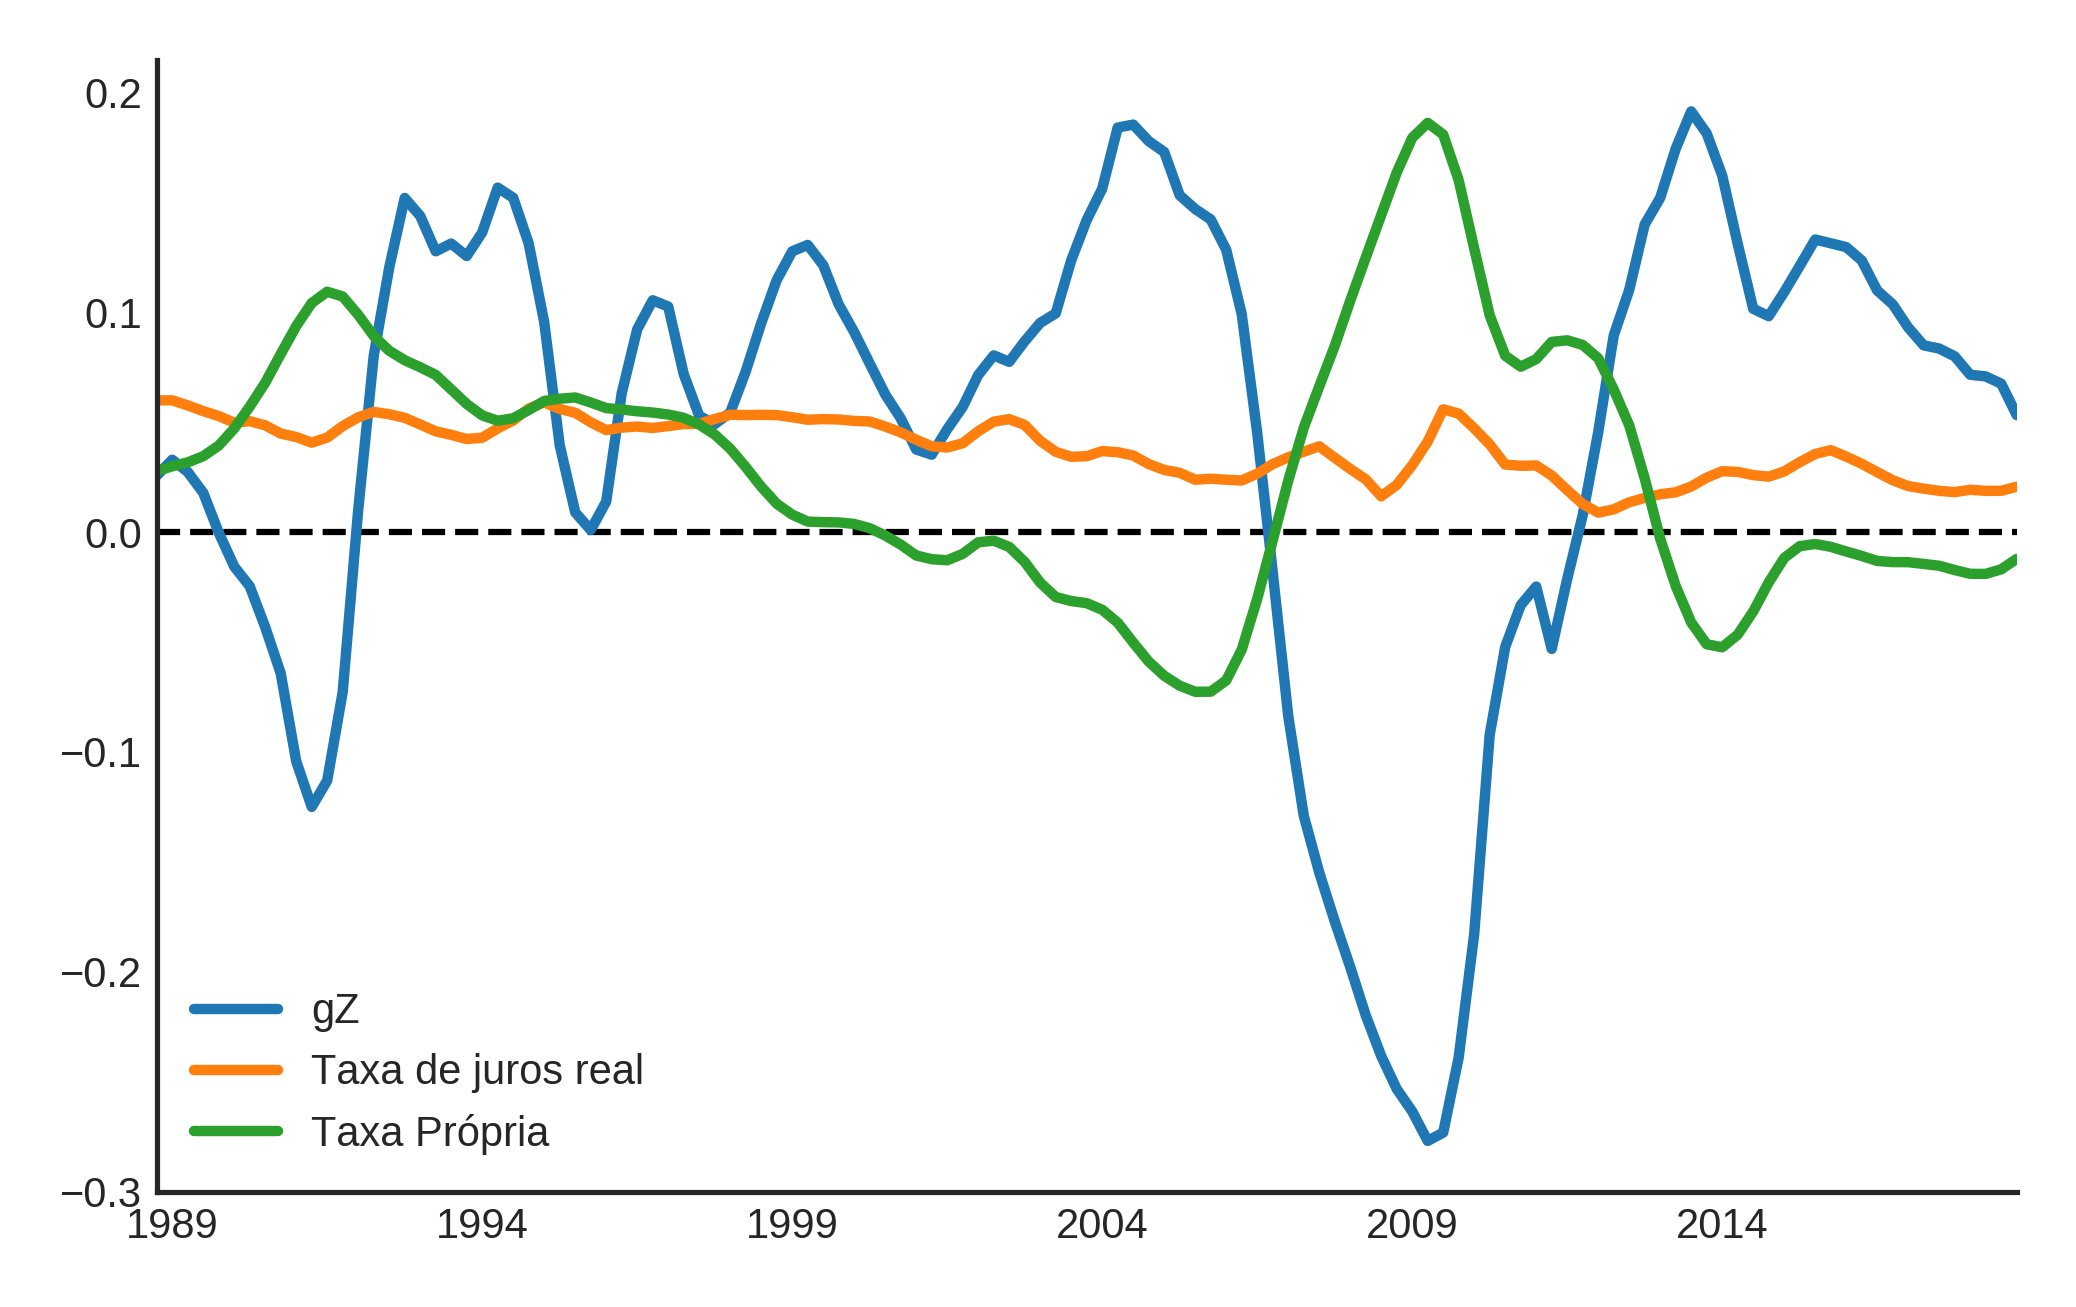
\includegraphics[width=0.75\textwidth]{Fatos_Estilizados/Figs/TxPropria_Investo.png}
	\caption*{\textbf{Fonte:} U.S. Bureau of Economic Analysis, elaboração própria}
\end{figure}
